\documentclass{article}
\usepackage{amsmath, sfmath, multicol, tkz-euclide, array, enumerate, tcolorbox, tabularray}
\renewcommand{\familydefault}{\sfdefault}
\setlength{\parindent}{0cm}
\pagestyle{empty}
\usepackage[left=1in, top=0.5in, right=1in, bottom=0.5in]{geometry}
\tikzset{>=stealth}
\tcbset{colback=white}

\newcounter{example}[section]
\newenvironment{example}[1][]{\refstepcounter{example}\par\medskip
   {\color{red}\textbf{Example~\theexample. #1}}}{\medskip}

\begin{document}

\section*{Congruence in Right Triangles}

\begin{tcolorbox}[colframe=orange!70!white, coltitle=black, title=\textbf{Today I Can}]
\begin{enumerate}
    \item Prove right triangles congruent using the hypotenuse-leg theorem.
\end{enumerate}
\end{tcolorbox}
\bigskip 

The \textbf{hypotenuse} of a right triangle is the side opposite the right angle.
\newline

The \textbf{legs} are the other two sides.

\begin{center}
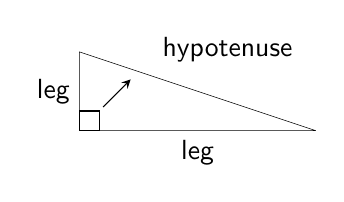
\begin{tikzpicture}
    \tkzDefPoints{0/0/A, 3/0/B, 0/1/C}
    \tkzDrawPolygon(A,B,C)
    \tkzMarkRightAngle(B,A,C)
    \draw[->, >=stealth] (0.3,0.3) -- (0.65,0.65);
    \tkzLabelSegment[left](A,C){leg}
    \tkzLabelSegment[below](A,B){leg}
    \tkzLabelSegment[above, xshift=0.15in, yshift=0.1in](B,C){hypotenuse}
\end{tikzpicture}
\end{center}

\begin{tcolorbox}[colframe=black!20!white, opacitybacktitle=0.1, coltitle=black, title=\textbf{Hypotenuse-Leg Theorem (HL)}]
If the hypotenuses and any pair of legs of two right triangles are congruent, then the triangles are congruent.
\newline

\begin{minipage}{0.3\textwidth}
\begin{itemize}
    \item $\triangle PQR \cong \triangle XYZ$
\end{itemize}
\end{minipage}
\begin{minipage}{0.6\textwidth}
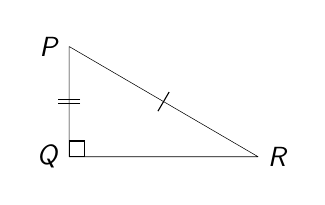
\begin{tikzpicture}[scale=0.8]
    \tkzDefPoints{0/0/Q, 0/1.75/P, 3/0/R}
    \tkzDrawPolygon(P,Q,R)
    \tkzLabelPoints[left](P,Q)
    \tkzLabelPoints[right](R)
    \tkzMarkSegment[mark=|](P,R)
    \tkzMarkSegment[mark=||](P,Q)
    \tkzMarkRightAngle(R,Q,P)
\end{tikzpicture}
\hspace{0.25in}
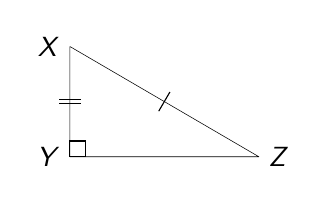
\begin{tikzpicture}[scale=0.8]
    \tkzDefPoints{0/0/Q, 0/1.75/P, 3/0/R}
    \tkzDrawPolygon(P,Q,R)
    \tkzLabelPoint[left](P){$X$}
    \tkzLabelPoint[left](Q){$Y$}
    \tkzLabelPoint[right](R){$Z$}
    \tkzMarkSegment[mark=|](P,R)
    \tkzMarkSegment[mark=||](P,Q)
    \tkzMarkRightAngle(R,Q,P)
\end{tikzpicture}
\end{minipage}
\end{tcolorbox}
\bigskip 

\textbf{Conditions for Hypotenuse-Leg}
\begin{itemize}
    \item There are 2 right triangles
    \item Triangles have congruent hypotenuses
    \item One pair of congruent legs
\end{itemize}
\bigskip 

\begin{example}
Prove each of the following.
\begin{enumerate}[(a)]
    \item \textbf{Given:} $\angle PRS$ and $\angle RPQ$ are right angles, $\overline{SP} \cong \overline{RQ}$ \quad \textbf{Prove:} $\triangle PRS \cong \triangle RPQ$ \newline\\

    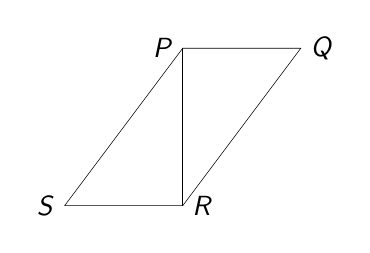
\begin{tikzpicture}
    \tkzDefPoints{0/0/S, 1.5/0/R, 1.5/2/P, 3/2/Q}
    \tkzDrawPolygon(S,R,Q,P)
    \tkzDrawSegment(P,R)
    \tkzLabelPoints[left](P,S)
    \tkzLabelPoints[right](R,Q)
    \end{tikzpicture}

    \newpage 

    \item \textbf{Given:} $\overline{BE} \text{ bisects } \overline{AD}, \, \overline{AB} \perp \overline{BC}, \, \overline{DE} \perp \overline{EC}, \, \overline{AB} \cong \overline{DE}$ \quad \textbf{Prove:} $\triangle ABC \cong \triangle DEC$ \newline\\

    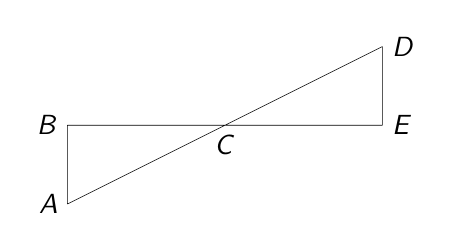
\begin{tikzpicture}
        \tkzDefPoints{0/0/B, 2/0/C, 4/0/E, 0/-1/A, 4/1/D}
        \tkzDrawPolygon(A,B,E,D)
        \tkzLabelPoints[left](A,B)
        \tkzLabelPoints[below](C)
        \tkzLabelPoints[right](D,E)
    \end{tikzpicture}

    \vfill 

    \item \textbf{Given:} $\overline{CD} \cong \overline{EA}, \, \overline{AD} \text{ is the perpendicular bisector of } \overline{CE}$ \quad \textbf{Prove:} $\triangle CBD \cong \triangle EBA$ \newline\\

    \begin{tikzpicture}
        \tkzDefPoints{0/0/A, 2/0/B, 4/0/D, 2/2/C, 2/-2/E}
        \tkzLabelPoints[left](A,C)
        \tkzLabelPoints[below](E)
        \tkzLabelPoints[right](D)
        \tkzLabelPoints[below right](B)
        \tkzDrawPolygon(A,D,C,E)
    \end{tikzpicture}
\end{enumerate}
\end{example}

\vfill 

\end{document}
